\documentclass[a4paper,12pt]{article} % тип документа

% Поля страниц
\usepackage[left=2.5cm,right=2.5cm,
    top=2cm,bottom=2cm,bindingoffset=0cm]{geometry}
    
%Пакет дял таблиц   
\usepackage{multirow} 
    
%Отступ после заголовка    
\usepackage{indentfirst}


% Рисунки
\usepackage{floatrow,graphicx,calc}
\usepackage{wrapfig}

%%% Работа с картинками
\usepackage{graphicx}  % Для вставки рисунков
\graphicspath{{images/}{images2/}}  % папки с картинками
\setlength\fboxsep{3pt} % Отступ рамки \fbox{} от рисунка
\setlength\fboxrule{1pt} % Толщина линий рамки \fbox{}
\usepackage{wrapfig} % Обтекание рисунков и таблиц текстом

% Создаёем новый разделитель
\DeclareFloatSeparators{mysep}{\hspace{1cm}}

% Ссылки?
\usepackage{hyperref}
\usepackage[rgb]{xcolor}
\hypersetup{				% Гиперссылки
    colorlinks=true,       	% false: ссылки в рамках
	urlcolor=blue          % на URL
}


%  Русский язык
\usepackage[T2A]{fontenc}			% кодировка
\usepackage[utf8]{inputenc}			% кодировка исходного текста
\usepackage[english,russian]{babel}	% локализация и переносы


% Математика
\usepackage{amsmath,amsfonts,amssymb,amsthm,mathtools}

%%% Дополнительная работа с математикой
\usepackage{amsmath,amsfonts,amssymb,amsthm,mathtools} % AMS
\usepackage{icomma} % "Умная" запятая: $0,2$ --- число, $0, 2$ --- перечисление


% Что-то 
\usepackage{wasysym}


\begin{document}
\begin{center}
	\footnotesize{ФЕДЕРАЛЬНОЕ ГОСУДАРСТВЕННОЕ АВТОНОМНОЕ ОБРАЗОВАТЕЛЬНОЕ 			УЧРЕЖДЕНИЕ ВЫСШЕГО ОБРАЗОВАНИЯ}\\
	\footnotesize{МОСКОВСКИЙ ФИЗИКО-ТЕХНИЧЕСКИЙ ИНСТИТУТ\\(НАЦИОНАЛЬНЫЙ 			ИССЛЕДОВАТЕЛЬСКИЙ УНИВЕРСИТЕТ)}\\
	\footnotesize{ФАКУЛЬТЕТ ОБЩЕЙ И ПРИКЛАДНОЙ ФИЗИКИ\\}
	\hfill \break
	\hfill \break
	\hfill \break
	\hfill \break
\end{center}


\begin{figure*}[h]
    \centering
    \includegraphics*[width=10cm,height=7cm,keepaspectratio]{mipt_eng_text_png.png}
    \label{fig:my_label}
\end{figure*}


\begin{center}   
    \hfill \break
	\hfill \break
	\hfill \break
	\hfill \break
	\large{Лабораторная работа № 1.3.3\\\textbf{Измерение вязкости воздуха по течению в тонких трубках}}\\
	\hfill \break
	\hfill \break
	\hfill \break
	\hfill \break
	\begin{flushright}
		Баранов Даниил\\
		Группа Б02-103
	\end{flushright}
	\hfill \break
	\hfill \break
	\hfill \break
\end{center}
\hfill \break
\hfill \break
\hfill \break
\hfill \break
\begin{center}
	Долгопрудный, 2022 г.
\end{center}
\thispagestyle{empty}



\newpage
\textbf{Цель работы:} экспериментально исследовать свойства течения газов по тонким трубкам при различных числах Рейнольдса; выявить область применимости закона Пуазейля и с его помощью определить коэффициент вязкости воздуха.\hfill
\break
	
\textbf{В работе используются:} система подачи воздуха (компрессор, поводящие трубки); газовый счетчик барабанного типа; спиртовой микроманометр с регулируемым наклоном; набор трубок различного диаметра с выходами для подсоединения микроманометра; секундомер.


\section{Теоретическая часть}
Рассмотрим движение вязкой жидкости или газа по трубке круглого сечения. При малых скоростях потока движение оказывается ламинарным (слоистым), скорости частиц меняются по радиусу и направлены вдоль оси трубки. С увеличением скорости потока движение становится турбулентным, а слои перемешиваются. При турбулентном движении скорость в каждой точке быстро меняет величину и направление, сохраняется только средняя величина скорости.

Характер движения газа (или жидкости) в трубке определяется безразмерным числом Рейнольдса:
\[
	Re = \frac{vr\rho}{\eta}
\]
где $v$ -- скорость потока, $r$ -- радиус трубки, $\rho$ -- плотность движущейся среды, $\eta$ -- её вязкость. В гладких трубах круглого сечения переход от ламининарного движения к турбулентному происходит при $Re \approx 1000$.

При ламинарном течении объем газа $V$, протекающий за время $t$ по трубе длиной $l$, определяется формулой Пуазейля:
\begin{equation}
	Q = \frac{\pi r^4}{8 \Delta l \eta}(P_1 - P_2)
\end{equation}
В этой формуле $P_1 - P_2$ -- разность давлений в двух выбранных сечениях 1 и 2, расстояние между которыми равно $\Delta l$. Величину $Q$ обычно называют расходом. Формула (1) позволяет определять вязкость газа по его расходу.

Отметим условия, при которых справедлива формула (1). Прежде всего необходимо, чтобы с достаточным запасом выполнялось неравенство $Re < 1000$. Необходимо также, чтобы при течении не происходило существенного изменения удельного объёма газа (при выводе формулы удельный объём считался постоянным). Для жидкости это предположение выполняется практически всегда, а для газа --- лишь в тех случаях, когда перепад давлений вдоль трубки мал по сравнению с самим давлением. В нашем случае давление газа равно атмосферному ($10^3$ см вод. ст.), а перепад давлений составляет не более 10 см вод. ст., т. е. менее 1\% от атмосферного. Формула (1) выводится для участков трубки, на которых закон распределения скоростей газа по сечению не меняется при двидении вдоль потока.
\begin{figure}[H]
\center
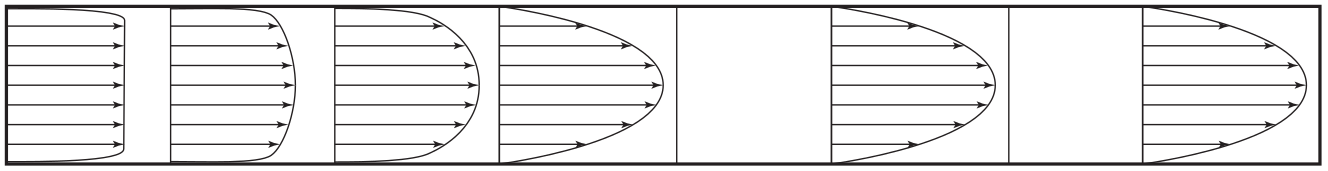
\includegraphics[scale=1]{potok.png}
\caption{Формирование потока газа в трубке круглого сечения}
\end{figure}
При втекании газа в трубку из большого резервуара скорости слоёв вначале постоянны по всему направлению. По мере продвижения газа по трубке картина распределения скоростей меняется, так как сила трения о стенку тормозит прилежащие к ней оси. Характерное для ламинарного течения параболическое распределение скоростей устанавливается на некотором расстоянии $a$ от входа в трубку, которое зависит от радиуса трубки $r$ и числа Рейнольдса по формуле 
\begin{equation}
	a \approx 0.2rRe
\end{equation}
Градиент давления на участке формирования потока оказывается больше, чем на участке с установившимся ламинарным течением, что позволяет разделить эти участки экспериментально. Формула (2) даёт возможность оценить дину участка формирования.

\section{Экспериментальная установка}

Схема экспериментальной установки изображена на Рис. \ref{233}. Поток воздуха
под давлением, немного превышающим атмосферное, поступает через газовый счётчик в тонкие металлические трубки. Воздух нагнетается компрессором, интенсивность его подачи регулируется краном К. Трубки снабжены
съёмными заглушками на концах и рядом миллиметровых отверстий, к которым можно подключать микроманометр. В рабочем состоянии открыта заглушка на одной (рабочей) трубке, микроманометр подключён к двум её выводам, а все остальные отверстия плотно закрыты пробками.

\begin{figure}[H]
    \centering
    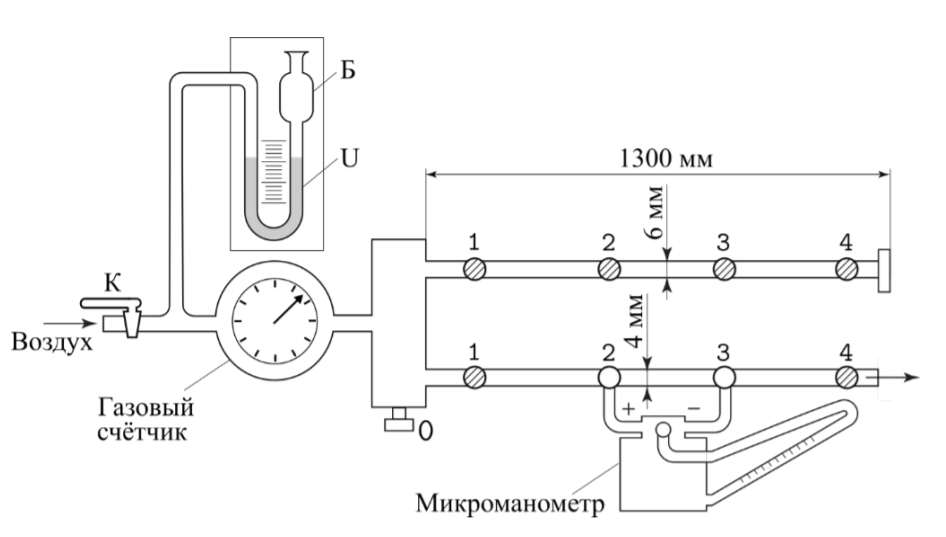
\includegraphics[scale=0.65]{1.3.3/expust.PNG}
    \caption{Экспериментальная установка}
    \label{233}
\end{figure}

Перед входом в газовый счётчик установлен водяной U-образный манометр. Он служит для измерения давления газа на входе, а также предохраняет
счётчик от выхода из строя. При превышении максимального избыточного
давления на входе счётчика ($\sim$ 30 см вод. ст.) вода выплёскивается из трубки
в защитный баллон Б, создавая шум и привлекая к себе внимание экспериментатора.


\textbf{Газовый счётчик.} В работе используется газовый счётчик барабанного
типа, позволяющий измерять объём газа $\Delta V$ прошедшего через систему. Измеряя время $\Delta t$ при помощи секундомера, можно вычислить средний объёмный расход газа $Q = \Delta V/ \Delta t$ (для получения массового расхода [кг/с] результат
необходимо домножить на плотность газа $\rho$).

\begin{figure}[H]
    \centering
    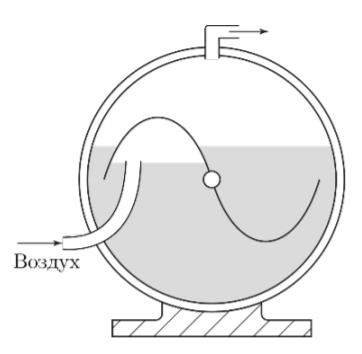
\includegraphics[scale=0.65]{1.3.3/gascounter.PNG}
    \caption{Газовый счетчик}
    \label{333}
\end{figure}


Работа счётчика основана на принципе вытеснения: на цилиндрической ёмкости жёстко
укреплены лёгкие чаши (см. Рис. \ref{333}, где для
упрощения изображены только две чаши), в которые поочередно поступает воздух из входной
трубки расходомера. Когда чаша наполняется,
она всплывает и её место занимает следующая
и т.д. Вращение оси предаётся на счётно-суммирующее устройство.
Для корректной работы счётчика он должен
быть заполнен водой и установлен горизонтально по уровню (подробнее см. техническое
описание установки).

\textbf{Микроманометр.} В работе используется жидкостный манометр с наклонной трубкой. Разность давлений на входах манометра измеряется по высоте
подъёма этилового спирта. Регулировка
наклона позволяет измерять давление в различных диапазонах.

На крышке прибора установлен трехходовой кран, имеющий два рабочих
положения — (0) и (+). В положении (0) производится установка мениска жидкости на ноль, что необходимо сделать перед началом работы (в процессе работы также рекомендуется периодически проверять положение нуля). В положении (+) производятся измерения.
\newpage


\section{Обработка рузультатов измерений}

Эксперимент проводился при комнатной температуре $T_\text{комн}=296,2 K$, при атмофсерном давлении $P_\text{атм}=101,75$ кПа и при относительной влажности в помещении $\eta=74\%$.

Давление, измеряемое микроманометром, определяется по формуле:
\[
P=9,81 \cdot K \cdot l 
\]
где $l$ -- показание макроманометра, $K$ -- коэффициент наклона, $P$ -- Давление в паскалях.

\subsection{Зависимость разности давлений от расхода}
Эксперимент проводился на первой трубе с диаметром $d_1=3,95\ \pm\ 0,05$ мм. Данные изменрений приведены в табилце \ref{tab:q(p)}.

\floatsetup[table]{capposition=top}
\begin{table}[H]
    \centering
    \begin{tabular}{|c|c|c|c|c|}
        \hline $h$, мм & $\Delta V$, л & $\Delta t$, с & $\Delta P$, Па & $Q$, мл$/$с \\
        \hline 15 & 3 & 153,4 & 29,4 & 19,6 \\
        \hline 22 & 3 & 103,5 & 43,1 & 29,0 \\
        \hline 29 & 3 & 81,0 & 56,8 & 37,5 \\
        \hline 35 & 4 & 91,0 & 68,6 & 44,4 \\
        \hline 41 & 3 & 58,1 & 80,4 & 51,7 \\
        \hline 49 & 3 & 49,1 & 96,0 & 61,1 \\
        \hline 57 & 4 & 56,8 & 111,8 & 70,4 \\
        \hline 64 & 4 & 51,0 & 125,6 & 78,4 \\ \hline
        \hline 80 & 5 & 53,3 & 156,8 & 93,8 \\
        \hline 87 & 5 & 50,8 & 170,5 & 98,4 \\
        \hline 100 & 7 & 66,9 & 196 & 104,6 \\
        \hline 119 & 8 & 72,9 & 233,2 & 109,7 \\
        \hline 162 & 8 & 66,4 & 317,5 & 120,5 \\
        \hline 196 & 8 & 61,8 & 384,2 & 129,4 \\
        \hline 234 & 9 & 63,8 & 458,6 & 141,0\\ \hline
    \end{tabular}
    \caption{Результаты измерений разности давлений от расхода}
    \label{tab:q(p)}
\end{table}

По результатам измерений был построен график \ref{p(q)}. По угловому коэффициенту и формуле (1) можно оценить вязкость воздуха. Она составила $\eta = 1,95 \pm 0,03 \times 10^{-5}$ Па$\cdot$с.

\begin{figure}[H]
    \centering
    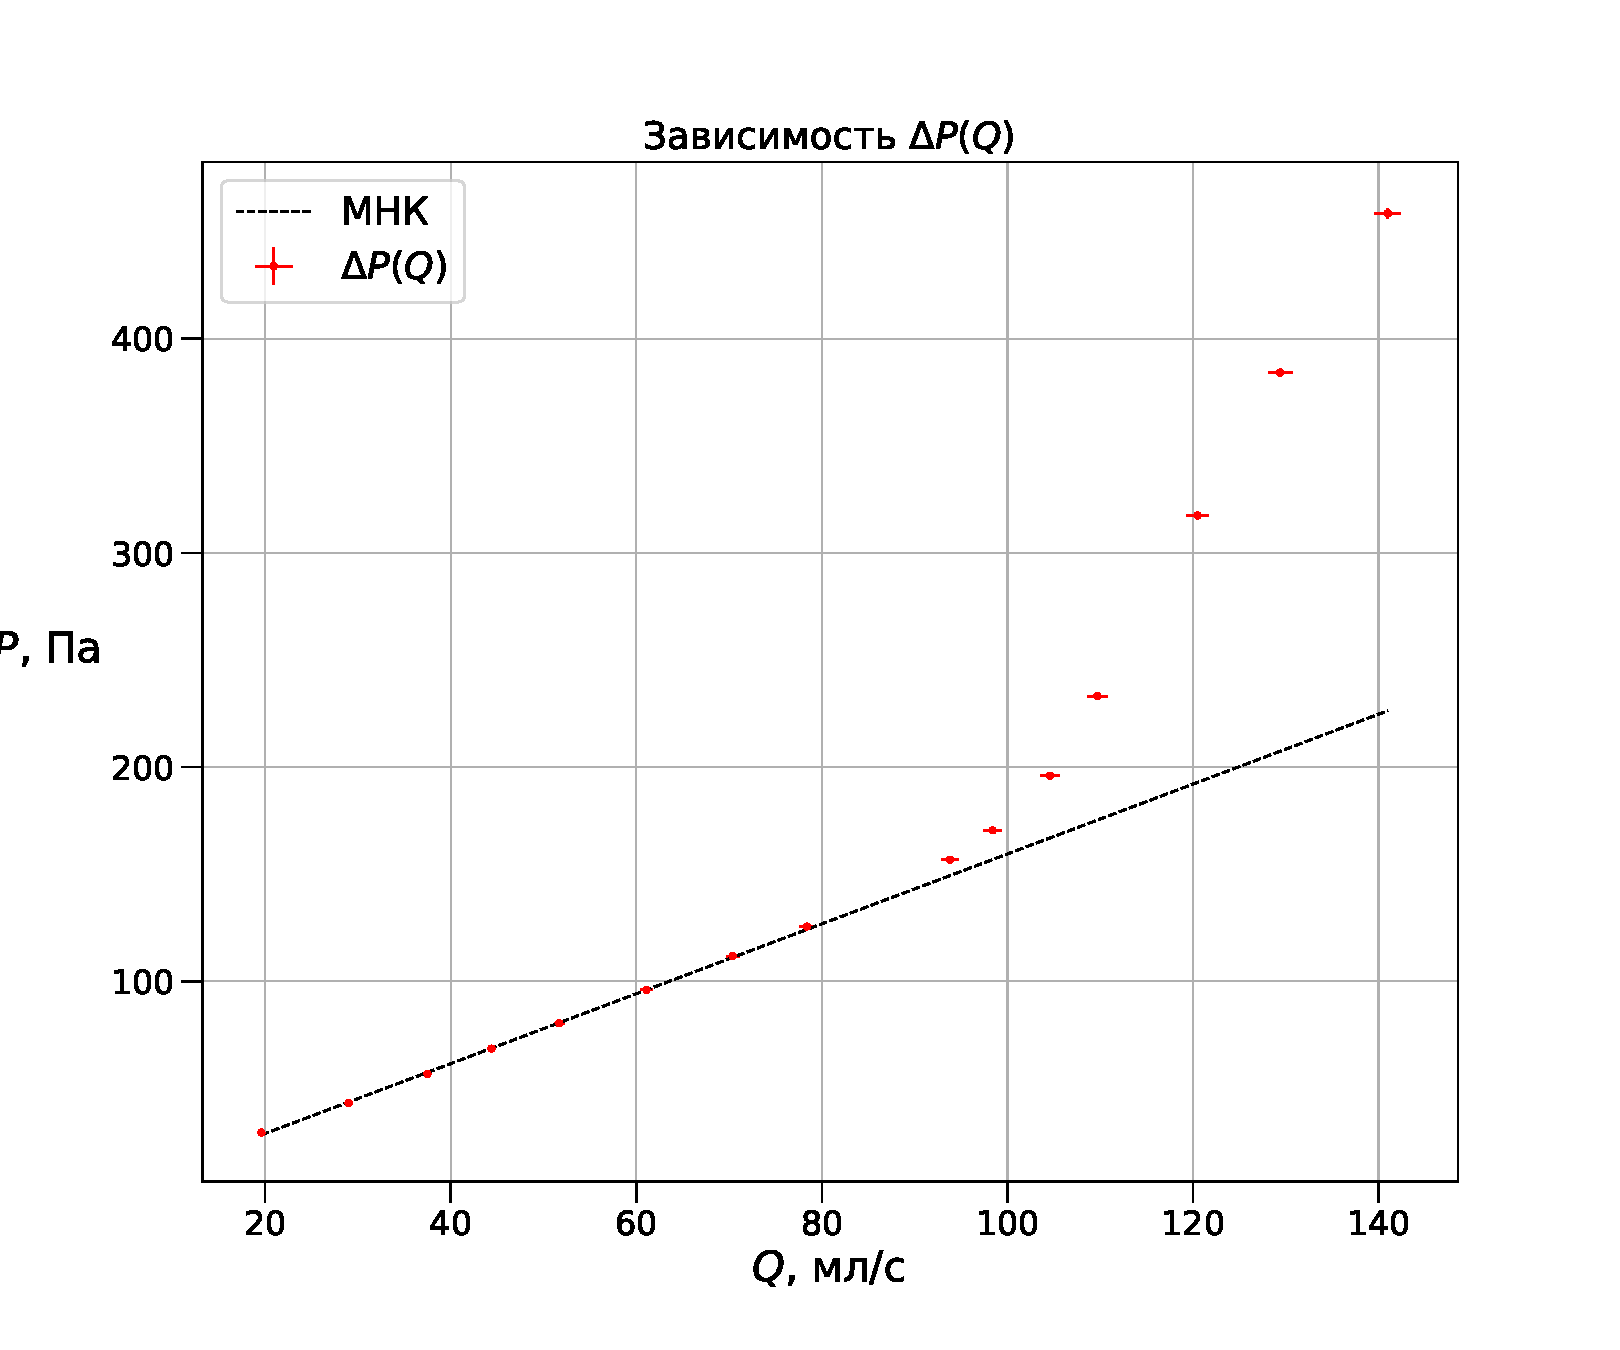
\includegraphics[scale=0.65]{p(q).pdf}
    \label{p(q)}
\end{figure}

\subsection{Зависимость разности давлений от длины участка}

Здесь измерения проводились на трубах 1 и 2 с диаметрами $d_1 = 3,95 \pm 0,05$ мм и $d_2 = 5,10 \pm 0,05$ мм, с расходами $Q_1 \approx 82,5$ мм/с и $Q_2 \approx 105,7$ мл/с соответственно.

\subsection{Зависимость разности давлений от длины}

Результаты измерений приведены в таблице \ref{p1}. По этим данным был построен график \ref{p(x)}, из которого следует, что ламинарное течение устанавливается не раньше 41 см.

\begin{table}[H]
    \centering
    \begin{tabular}{|c|c|}
        \hline \multicolumn{2}{|c|}{$Q=82,5$ мл/с, $d=3,95$ мм} \\ \hline
        $x$, см & $\Delta P$, Па \\ \hline
        10,9 &  82,3 \\ \hline
        40,9 &  186,2 \\ \hline
        80,9 &  313,6 \\ \hline
        130,9 & 450,8 \\ \hline
        \multicolumn{2}{c}{} \\
        \hline \multicolumn{2}{|c|}{$Q=105,7$ мл/с, $d=5,10$ мм} \\ \hline
        10,9 &  52,9 \\ \hline
        40,9 &  94,1 \\ \hline
        80,9 &  121,5 \\ \hline
        130,9 & 182,3 \\ \hline
    \end{tabular}
    \caption{Зависимость давления от длины}
    \label{p1}

\end{table}

\begin{figure}[H]
    \centering
    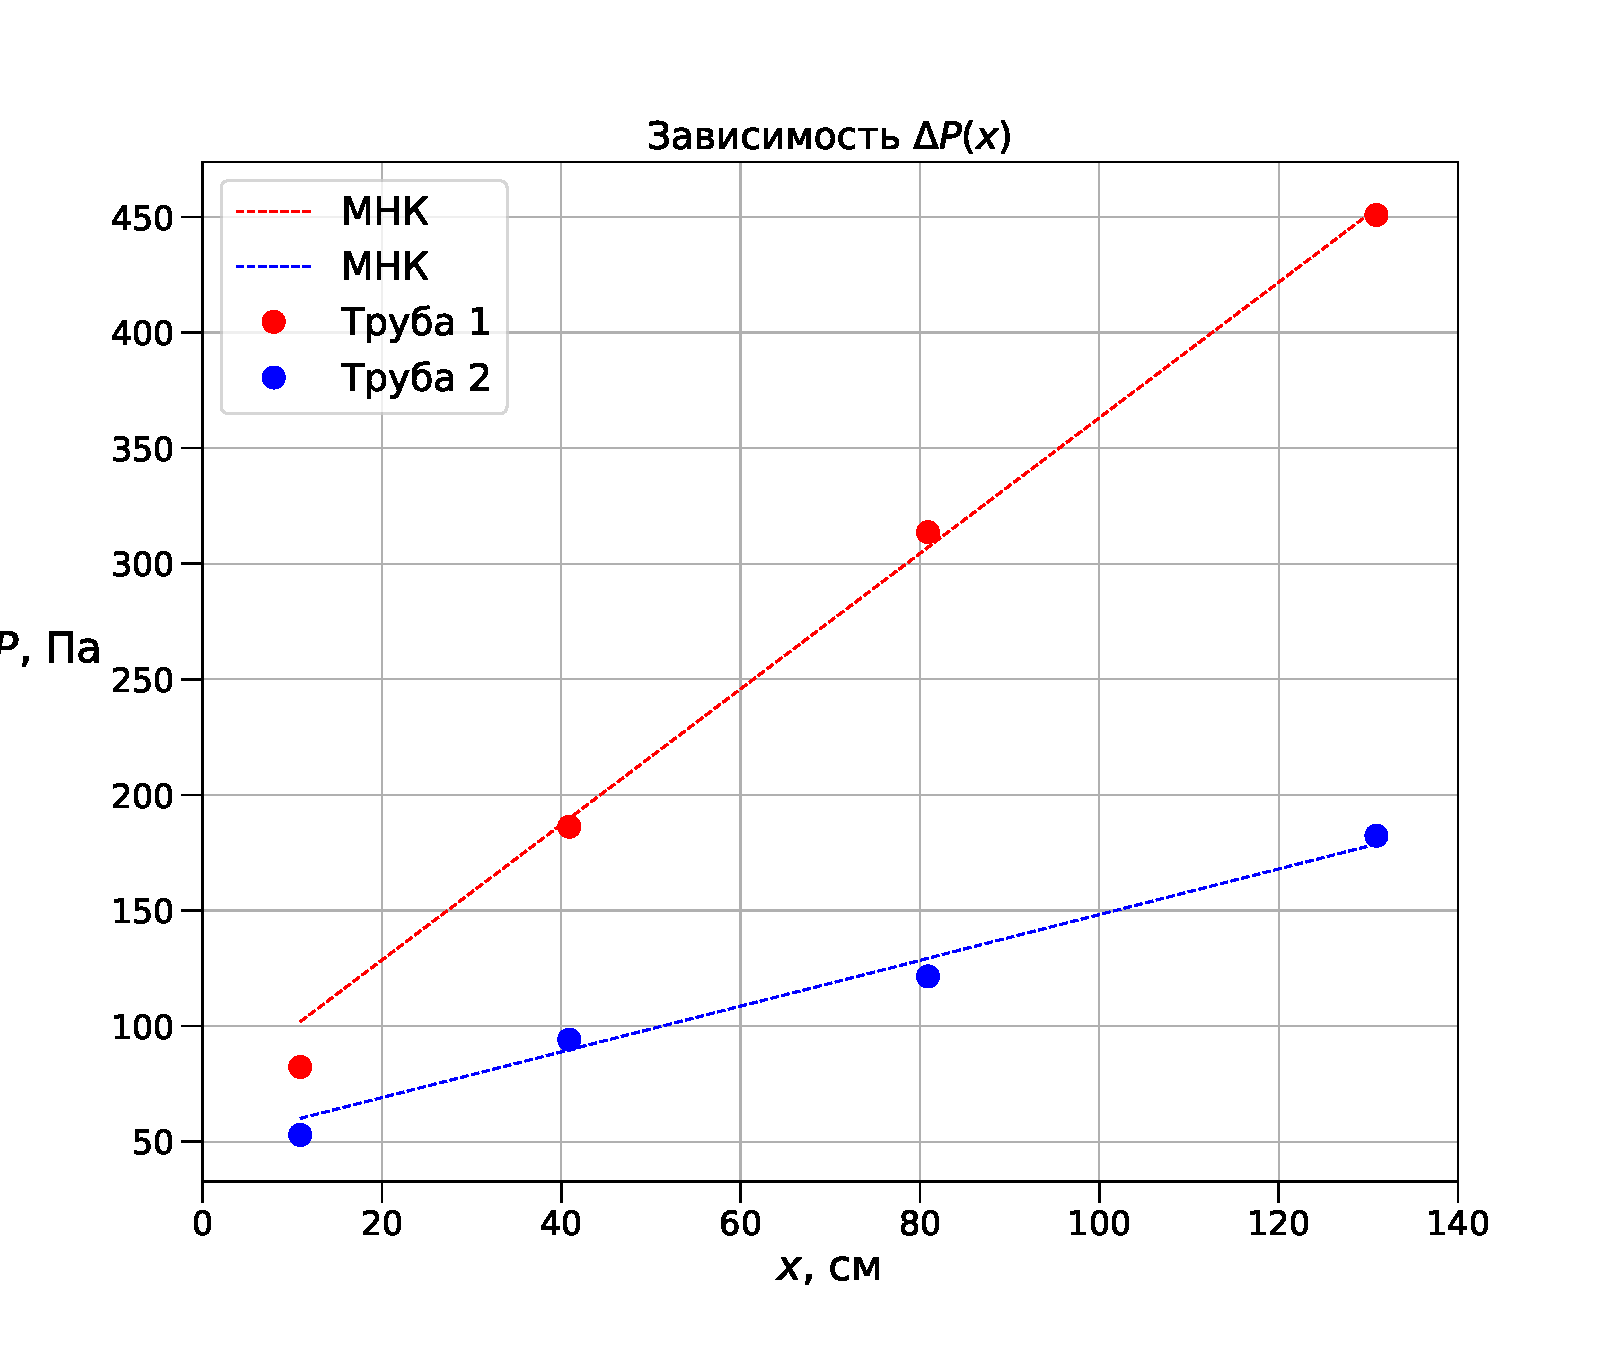
\includegraphics[scale=0.65]{p(x).pdf}
    \label{p(x)}
    \caption{Зависимость разности давлений от длины}
\end{figure}

\subsection{Зависимость расхода от диаметра трубы}

Данные измерений приведены в таблицах. Для измерения зависимости в ламинарном течении было выбрано значение $dP/dl = 0,98$ Па/см. Для турбулентного течения -- $dP/dl = 6,27$ Па/см.


\begin{table}[H]
    \centering
    \begin{tabular}{|c|c|}
    \hline \multicolumn{2}{|c|}{Ламинарное теч.} \\
        \hline $Q$, мл/с & $d$, мм \\ \hline
        31 & 3,95 \\ \hline
        11,5 & 3 \\ \hline
        105,7 &  5,10 \\ \hline
        \multicolumn{2}{c}{} \\ \hline
        \multicolumn{2}{|c|}{Турбулентное теч.} \\ \hline
        $Q$, мл/с & $d$, мм \\ \hline
        119 & 3,95 \\ \hline
        57,7 & 3 \\ \hline
        268,8 &  5,10 \\ \hline
    \end{tabular}
    \caption{Зависимость расхода от градиента давления}
\end{table}




Из графика видно, что для турбулентного течения всё выполняется хорошо и расход пропорционален радиусу в степени 2,5. С ламинарным же течение зависимость не подтвердилать, показав степень 3,5. Это может говорить о неправильном теоретическом приближении.

\begin{figure}[H]
    \centering
    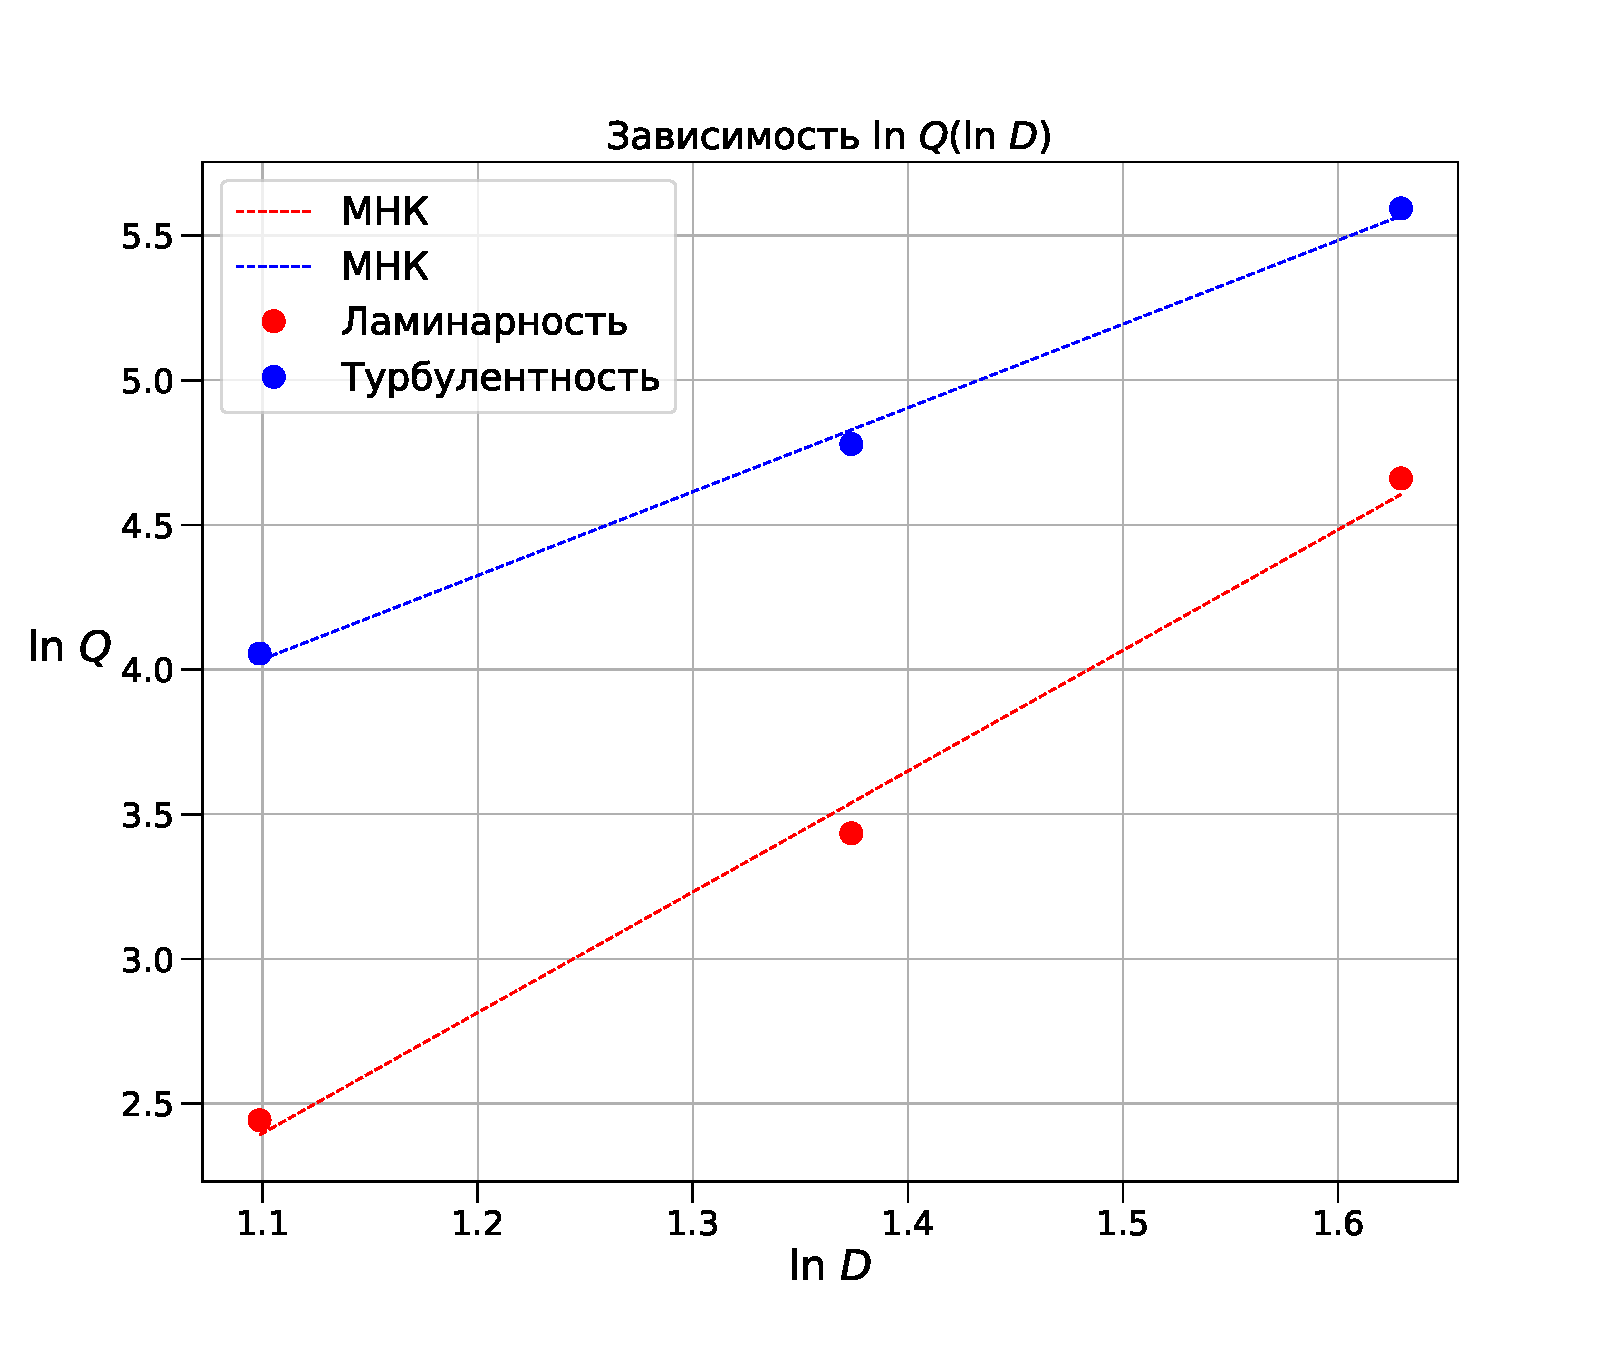
\includegraphics[scale=0.65]{q(d).pdf}
    \label{q(d)}
    \caption{Зависимость расхода от градиента давления}
\end{figure}


\end{document}
